%mscS --> seminar
%msc --> Thesis

% برای گزارش سمینار mscS  و برای پایان‌نامه ,msc را انتخاب کنید
\documentclass[oneside,openany,mscS]{SBU-Thesis}

% برای وارد کردن بسته‌هایی که نیاز است قبل از bidi وارد شوند، آنها را در فایل confix.tex قرار دهید. سایر بسته‌های مورد نیاز را در اینجا می‌توانید وارد کنید:

\begin{document}
	%عنوان پایان‌نامه
	\title{کاهش شروع‌های سرد در پلتفرم‌های بدون سرور}
	
	%رشته
	\subject{مهندسی کامپیوتر}
	
	%گرایش
	\field{نرم‌افزار}
	
	%نام
	\name{امیرمحمد}
	
	%نام خانوادگی
	\surname{کرم‌زاده}

	%استاد مشاور (در صورت وجود، در غیر این صورت این خط را حذف کنید)
	\firstsupervisor{دکتر علیرضا شاملی}

%تاریخ انجام پایان‌نامه
	\thesisdate{خرداد 1400}
	
	%نام دانشکده
	\faculty{دانشکده مهندسی و علوم کامپیوتر}
	
	%نام دانشگاه
	\university{دانشگاه شهید بهشتی}

	% چکیده به فارسی
	\fa-abstract{رایانش ابری، یکی از مباحث داغ حوزه مهندسی نرم‌افزار است که به دلیل فواید بسیار آن، مورد توجه کاربران قرار گرفته است. یکی از مدل‌های اجرایی در رایانش ابری، مدل اجرایی رایانش بدون سرور است که با هدف راحتی کاربران و توسعه‌دهندگان برنامه‌ها و ابزارها برای توسعه‌ی خدمات ابری، برنامه‌های کاربردی در وب یا برنامه‌های کاربردی موبایل طراحی شده است. اگرچه رایانش بدون سرور با ساده‌سازی فرآیند تعامل و مدیریت،‌ بسیار موفق عمل کرده است؛ اما، این مدل اشکلاتی دارد که مانع تمایل کاربرا به سمت آن شده است. رایج‌ترین معضل کاربران با پلتفرم‌ّهای بدون سرور تاخیر ناشی از پاسخ برنامه‌هاست که به تاخیر شروع سرد معروف است. این تاخیر می‌تواند در مواردی زمان پاسخ را تا چندین برابر افزایش دهد و معمولا چندین برابر زمان اجرای برنامه است. بنابراین لازم است که با این مشکل به صورت جدی مقابله شود. ما متوجه‌ شدیم عمده تاخیر ناشی از شروع سرد به علت آماده سازی کانتینر‌های سرویس فراخوانی شده و بارگذاری کتابخانه‌های برنامه‌نوشته شده در داخل کانتینر هستند. البته بعد از این کارها باید منابع کافی (RAM و CPU) برای اختصاص به کانتینر داشته باشیم. برای مقابله با شروع سرد، دو راهکار کلی داریم. راهکار اول این است که مانع از اتفاق افتادن شروع سرد شویم و راهکار دوم بهبود زمان شروع سرد است. این دو هر کدام مزیت و عیب خود را دارند که در x در مورد آن بحث‌هایی خواهد شد. در x به این نتیجه رسیدیم که احتمالا بتوانیم با ترکیب مدل‌هایی بتوانیم مانع از شروع‌های سرد بشویم.  به طور خلاصه پژوهش ما درباره‌ی حداقل سازی شروع سرد و راهکار‌های کمینه سازی آن است. }
	%کلمات کلیدی:
	\keywords{رایانش ابری، رایانش بدون سرور، شروع‌های سرد، \lr{function-as-a-service}، \lr{FaaS}}
	%%%%%%%%%%%%%%%%%%%%%%%%%%%%%%%%%

%%%%%%%%%%%%%%%%%%%%%
\firstPage
\abstractPage % ساخت صفحه چکیده


\tableofcontents % فهرست مطالب
\listoffigures \newpage % فهرست تصاویر
\listoftables \newpage % فهرست جداول

%%%%%%%%%%%%%%%%%%%%%%%%%%%

\cchapter{مقدمه}

\section{صورت مسئله}
\par 
چه روش‌هایی برای کاهش تعداد شروع‌های سرد در پلتفرم‌های بدون‌سرور \LTRfootnote{serverless} با حداقل سربار \LTRfootnote{Overhead} و زمان اجرایی وجود دارند؟ 

\section{انگیزه‌ی تحقیق}
\par
رایانش بدون سرور\LTRfootnote{Serverless Computing} یکی از مسائل داغ و محبوب این‌روز‌های دنیای مهندسی نرم‌افزار و رایانش ابری است. رایانش بدون سرور حوزه‌ی جدیدی را در توسعه‌ی محصول و استقرار\LTRfootnote{Deployment} اپلیکیشن‌ها باز کرده است. یکی از دلایل محبوبیت استفاده از پلتفرم‌های بدون‌سرور و تمایل توسعه‌دهندگان برای مهاجرت به سمت آن، استفاده بیش از پیش از معماری میکروسرویس و نانوسرویس در توسعه‌ی محصولات و حرکت معماران و مهندسین نرم‌افزار در تولید و مهاجرت برنامه‌های کاربردی با این معماری‌ها است.

\par 
از دید توسعه دهنده، رایانش ابری با حذف دخالت مستقیم کاربران انتهایی در مدیریت زیرساخت ازجمله lr{auto-scaling} یا lr{load-balancing} موجب بهبود سرعت توسعه محصول و تمرکز کاربران برروی منطق\LTRfootnote{logic} برنامه است. همچنین، برای علاوه‌بر آسانی استفاده و پنهان‌سازی پیچیدگی مدیریت سرور از کاربر، به علت اینکه ارائه‌دهندگان خدمات ابری در نقاط مختلف جهان حضور دارند و همچنین کانفیگ بهینه \lr{CDN}ها؛  ارتباطات بین سرورها و کاربران با حداقل تاخیر\LTRfootnote{Latency} صورت می‌گیرد. 

\par
به طور کلی، یک‌ پلتفرم بدون‌سرور را هر پلتفرم محاسباتی تعریف کرد که در آن مدیریت مستقیم سرور از کاربران مخفی شده و برنامه‌های کاربردی به صورت اتوماتیک در آن مقیاس‌پذیر می‌شوند و تنها هنگامی که در حال استفاده از پلتفرم هستیم، هزینه آن را پرداخت می‌کنیم. \cite{The_Rise_of_Serverless_Computing}

\par 
یکی از قابلیت‌هایی که در رایانش بدون سرور باعث محبوبیت آن شده‌است، قابلیت \lr{Scale-to-Zero} است. این بدان معنی است که هنگامی که از یک کانتینر استفاده‌ای نداریم، منابع آن گرفته‌ می‌شوند و کانتینر اصطلاحا \lr{Zero-Scaled} می‌شود. این خود موجب قابلیت پرداخت تنها در حین مصرف ما از تابع می‌شود. اما مشکل اصلی زمانی است که درخواست جدیدی برای کانینر \lr{Zero-Scale} شده می‌رسد؛ در این حالت باید درخواست منتظر مانده تا سلسله‌ای از آماده‌سازی ها انجام شوند تا کانتینر مربوطه مجددا اجرا شود. این خود باعث تاخیری مضاف برای پاسخ‌دهی به درخواست را موجب می‌شود که به این تاخیر مشکل شروع‌سرد  \LTRfootnote{Cold Start} گفته می‌شود. در واقع می‌توان گفت تاخیر شروع سرد ناشی از تلاش ما در تعادل بین تاخیر در پاسخگویی به درخواست‌ها و هزینه (هزینه‌های استفاده از رم و سی‌پی‌یو و …) است.

\par
متاسفانه در سالیان اخیر و در عین داغ‌بودن مبحث و نیاز بازار به حل این مشکل، این مشکل چندان در محیط‌های آکادمیک مورد بررسی قرار نگرفته است. البته در نگاه کلی‌تر، مشکلات و مسائل بار مربوط به رایانش بدون‌سرور، اکثرا در محیط‌های آکادمیکی مثل دانشگاه‌ها با کم محلی روبرو شده‌اند. در این میان، پلتفرم‌های متن‌باز\LTRfootnote{Open Source} که دارای جوامع بسیار گسترده‌ای نیز هستند، به خاطر این سری مسائل باز که شرکت‌‌های تجاری در حال صرف هزینه‌های هنگفتی برای حل و فصل مسکلات مربوط‌ به آن‌ هستند، به شدت از رقابت عقب مانده‌اند. انگیزه ما برای انجام این پژوهش در این است که اولا بتوانیم به راهکار مناسب‌تری برای حل مشکل مربوط به شروع سرد در پلتفرم‌های بدون سرور برسیم و ثانیا بتوانیم با مشارکت در بهبود یکی از پلتفرم‌های آزاد در توسعه این پلتفرم‌ها تاثیر کوچکی داشته باشیم. 


\section{مثال مرتبط}
\par

در مقاله \cite{lin2019mitigating} آقای لین و همکارش توانستند تا با اسفاده از استخر گرم و نگه‌داری کانتینر توابعی که محبوبیت استفاده دارند، مدت زمان پاسخ را در حدود 85٪ کاهش دهند. این بهبود در پلتفرم \lr{knative} اجرا شد و ایده‌ی مقالات دیگری نیز بوده است.

\section{اهمیت موضوع}
\par 

اگرچه پلتفرم‌های بدون‌سرور از نظر هزینه، \lr{scaling}، راحتی استفاده و گستردگی پوشش جغرافیایی برای ما بهینه هستند؛ اما مشکل شروع سرد مشکلی نیست که بتوان به سادگی از آن گذر کرد. 
تصویر \ref{fig:coldstart-importance} که از \cite{mohan2019agile} گرفته شده است، نشان می‌دهد که بیش از 80٪ زمان اجرای کامل یک کانتینر در پلتفرم‌های بدون سرور به آماده‌سازی آن یا شروع سرد اولیه\LTRfootnote{First Cold Start} مربوط می‌شود. 

\begin{figure}
	\centering
	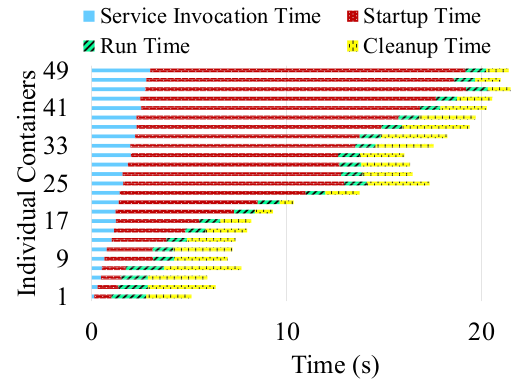
\includegraphics[width=\linewidth]{figs/coldstart-importance}
	\caption {اهمیت شروع‌سرد}
	\label{fig:coldstart-importance}
\end{figure}

\par
ستون قرمز رنگ زمان آماده سازی کانتینر را نمایش می‌دهد. این زمان همان زمان شروع سرد است که دلایل مختلفی از جمله آماده‌سازی کانتینر یا حضور در صف انتظار برای تخصیص منابع باشد. بنابراین، با به‌کارگیری یک استراتژی مناسب می‌توان این زمان را به حداقل رسانید. 

\par 
متاسفانه تاخیر شروع سرد باعث شده تا توسعه‌دهندگان اقبال کمتری به استفاده از پلتفرم‌های بدون سرور داشته باشند. به گونه‌ای که از بین 1000 برنامه‌ی کاربردی بزرگ در پلتفرم \lr{Microsoft Azure}، تنها یک مورد مربوط به یک برنامه تجاری باشد\cite{shahrad2020serverless}. این موضوع  نشان می‌دهد که علی‌رغم پتانسیل بالای رایانش بدون سرور، وجود مشکلات جدی ازجمله شروع سرد، باعث امتناع توسعه‌دهندگان از مهاجرت به پلتفرم‌های بدون سرور باشد. 

\par 
\section{نتیجه‌های مهم تحقیق}
لورم ایپسوم متن ساختگی با تولید سادگی نامفهوم از صنعت چاپ، و با استفاده از طراحان گرافیک است، چاپگرها و متون بلکه روزنامه و مجله در ستون و سطرآنچنان که لازم است، و برای شرایط فعلی تکنولوژی مورد نیاز، و کاربردهای متنوع با هدف بهبود ابزارهای کاربردی می باشد، کتابهای زیادی در شصت و سه درصد گذشته حال و آینده، شناخت فراوان جامعه و متخصصان را می طلبد، تا با نرم افزارها شناخت بیشتری را برای طراحان رایانه ای علی الخصوص طراحان خلاقی، و فرهنگ پیشرو در زبان فارسی ایجاد کرد، در این صورت می توان امید داشت که تمام و دشواری موجود در ارائه راهکارها، و شرایط سخت تایپ به پایان رسد و زمان مورد نیاز شامل حروفچینی دستاوردهای اصلی، و جوابگوی سوالات پیوسته اهل دنیای موجود طراحی اساسا مورد استفاده قرار گیرد.

\par
\par
ساختار این گزارش به این ترتیب خواهد بود:‌

‫در\hyperref[literature] {ادبیات موضوع} مروری بر واژگان، مفاهیم تخصصی و هر آن‌چه که در ادامه به آن نیاز پیدا خواهیم کرد، خواهیم داشت. سپس در فصل
\hyperref[related-works]{کار‌های مرتبط}
  به بیان مشروح تحقیقات انجام شده خواهیم پرداخت و در  
\hyperref[conclusion]{نتیجه‌گیری و کار‌های آینده}
  خلاصه‌ای از مطالعات انجام شده و مسائل باز خواهیم پرداخت. ‬
\cchapter{مروری بر ادبیات}
\label{literature}
در این بخش سعی داریم تا با مروری بر اصطلاحات و ابزارهای مورد استفاده در پژوهش‌های بررسی شده، با پیش‌نیازهای مبحث موردنظر آشنا شویم. 
\section{رایانش بدون سرور}
رایانش بدون سرور\LTRfootnote{Serverless Computing} در سال 2014 توسط شرکت آمازون برای اولین بار معرفی شد. تا قبل از این رایانش بدون سرور یک مفهوم انتزاعی \LTRfootnote{abstract} در شبکه بود که شرکت آمازون با ارائه پلتفرم \lr{AWS Lambda Functions} \cite{aws} به معرفی آن پرداخت. سپس در سال 2016 سایر ارائه دهندگان خدمات ابری نیز به ارائه پلتفرم‌های بدون سرور خود پرداختند. در این سال به ترتیب شرکت‌های گوگل پلتفرم \lr{google cloud functions} یا به اختصار \lr{GCP}، شرکت مایکروسافت پلتفرم \lr{Microsoft Azure functions} و شرکت \lr{IBM} به معرفی \lr{IBM OpenWhisk} پرداختند. البته باید توجه داشت که مفهوم رایانش بدون سرور به طور کامل توسط ارائه دهندگاه خدمات ابری پیاده‌سازی نشده است و جای کار بسیاری دارد (با مطالعه این گزارش به مرور متوجه نواقص موجود خواهید شد).

در رایانش بدون سرور ما از نقطه قوت ماشین‌های مجازی که ایزولاسیون برنامه‌های مختلف از همدیگر بود استفاده کرده‌ایم. منتها این مورد را با مفهوم کانتینر ها پیاده‌کرده ایم. در ادامه راجع به کانتینرها نیز بحث خواهیم کرد. 

\subsection{تعریف رایانش بدون سرور}
\par
رایانش بدون سرور مبحثی از رایانش ابری است که در آن بحث مدیریت حافظه یا \lr{Storage}، مدیریت زیرساخت و بحث‌های \lr{networking} با انتزاع بالایی به مصرف کاربر می‌رسد. به عبارت دیگر، تمامی مدیریت ای بخش‌ها بر عهده ارائه دهندگان است و ما اصلا با این بحث ها سروکاری نداریم. در واقع، هدف اصلی رایانش بدون سرور هم این است که این پیچیدگی‌ها را از کاربر بگیرد. 

\par
به طور کلی، یک‌ پلتفرم بدون‌سرور را هر پلتفرم محاسباتی تعریف کرد که در آن مدیریت مستقیم سرور از کاربران مخفی شده و برنامه‌های کاربردی به صورت اتوماتیک در آن مقیاس‌پذیر می‌شوند و تنها هنگامی که در حال استفاده از پلتفرم هستیم، هزینه آن را پرداخت می‌کنیم. \cite{The_Rise_of_Serverless_Computing}

\par
بسیاری از افراد، \lr{serverless} و \lr{faas} را معادل یک‌دیگر می‌دانند درحالی‌که اصلا این‌گونه نیست. در ادامه راجع به این بحث به طور مفصلی بحث خواهیم کرد اما باید بدانیم که این دو مقوله کاملا جدا از همدگیر هستند و مجددا تاکید می‌کنیم که رایانش بدون سرور یک مدل اجرایی در رایانش ابری است. 

\par
ازطرفی رایانش بدون سرور را باید نقطه مقابل رایانش سرور آگاهانه \LTRfootnote{Server Aware} دانست که در آن از اطلاعات سرور در اختیار گرفته کاملا اگاهیم، کاملا بر مدیریت آن اشراف داریم و هرگونه تغییر از جمله متعادل‌سازی بارها، \lr{auto-scaling} و … باید توسط کاربر انجام شود.

\par
یک مثال از پیاده‌سازی رایانش سرور آگاهانه را در زیرساخت به عنوان سرویس \LTRfootnote{Infrastructure as a service} یا به اختصار \lr{IaaS} است. در نقطه مقابل در رایانش بدون سرور هیچ کنترلی بر روی سرور نداریم، تنها می‌توانیم یک برنامه را بر روی سرور اجرا کنیم یا اجرای آن را به حالت تعلیق درآورده یا آن را از روی سرور حذف کنیم که هیچ‌کدما از این موارد نیز به صورت مستقیم انجام نمی‌گیرد؛ بلکه رابط گرافیکی و \lr{API} وجود دارد که از طریق آن‌‌ها این تغییرات را اعمال می‌کنیم. بنابراین در رایانش بدون سرور، عملا هیچ راهی برای مدیریت مستقیم سرور و زیرساخت نداریم.

شکل \ref{fig:ServerlessVSServeraware} مرز‌های بین رایانش بدون‌سرور و رایانش سرور آگاهانه را نمایش می‌دهد.  

\begin{figure}
	\centering
	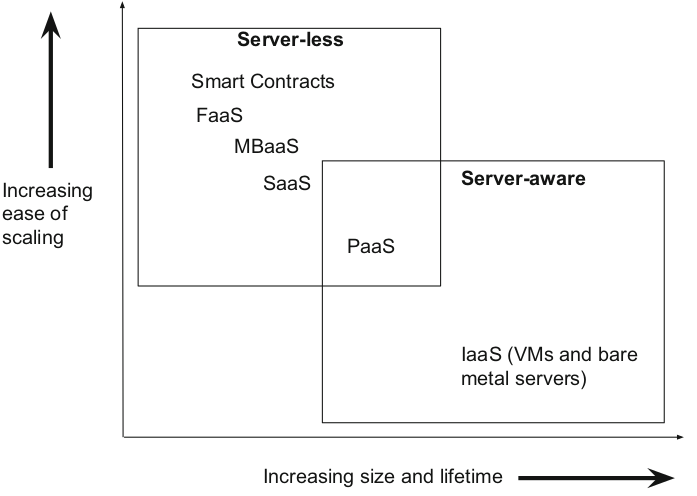
\includegraphics[width=\linewidth]{figs/ServerlessVSServeraware}
	\caption {مرز‌های رایانش بدون سرور و رایانش سرورآگاهانه}
	\label{fig:ServerlessVSServeraware}
\end{figure}

\par
البته باید به این نکته توجه‌داشت که امروزه مرز‌های بین رایانش سرور آگاهانه با رایانش بدون سرور در حال کمرنگ شدن و بعضا از بین رفتن است و این تقسیم بندی ابدا قاطعیت ندارد.همچنین تفکیک برخی موارد مانند \lr{Platform-as-a-Serice} یا به اختصار \lr{PaaS} به راحتی انجام نمی‌گیرد بلکه این نوع رایانش می‌تواند از نوع باسرور یا بدون سرور باشد. 
در این شکل هرچه به سمت محور افقی حرکت می‌کنیم دانه‌بندی و طول‌عمر افزایش پیدا می‌کند و هرچه به سمت بالاتر می‌رویم، \lr{scalingz} راحت‌تر انجام می‌گیرد. 

\par
از مزایای رایانش بدون سرور همچنین می‌توان به پشتیبانی و توسعه راحت‌تر اپلیکیشن‌ها با معماری میکروسرویس و نانوسرویس هم اشاره کرد. البته معماری نانوسرویس مبحث جدیدتری است و جای پژوهش‌های بیشتری دارد.

\subsection{معماری}
\par
واژه serverless ممکن است این تفکر را به ذهن مبتدر سازد که اصلا در این نوع مدل رایانشی سروری نداریم؛ در حالی‌که این امر بسیار اشتباه است. در رایانش بدون سرور اگرچه سروری برای مدیریت به کاربر اختصاص داده نمی‌شود اما این موضوع بدان معنا نیست که اصلا سروری در کار نیست. در واقع مانند تمامی مدل‌های رایانشی در این‌جا هم سرور داریم، ولی تمامی تصمیمات مثل توزیع بار، تعداد اپ‌های روی سرور، انتخاب سرور‌ها برای اجرای اپلیکیشن، کانفیگ CI/CD و … بر عهده ارائه دهنده خدمات ابری است. اما برای درک نحوه کار یک پلتفرم بدون سرور، بهتر است با معماری آن آشنا باشیم. شکل \ref{fig:Serverless-Architecture} معماری یک پلتفرم خدمات ابری را نشان می‌دهد.

\par

\begin{figure}
	\centering
	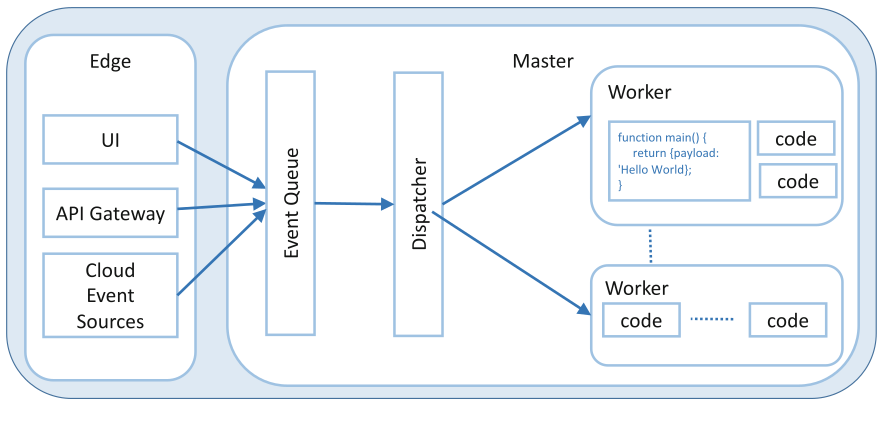
\includegraphics[width=\linewidth]{figs/Serverless-Architecture}
	\caption {معماری کلی یک پلتفرم بدون سرور}\LTRfootnote{Serverless Platform Architecture}
	\label{fig:Serverless-Architecture}
\end{figure}

\par
همانگونه که در تصویر مشخص است دوبخش کلی داریم، بخش لبه\LTRfootnote{edge}‌ و بخش رییس \LTRfootnote{master}، بخش لبه شامل رابط گرافیکی کاربر\LTRfootnote{User Interface}، API Gateway و \lr{Cloud Event Source} می‌شود که برای تعامل با سرور رییس\LTRfootnote{master server} مناسب هستند. از طرف دیگر، در سرور رییس، درخواست‌ها ابتدا به صف رخداد‌ها\LTRfootnote{Event Queue} رسیده. صف رخداد‌ها مسئول مدیریت رخداد و نظم‌دهی به آن‌ّ‌ها است. هر داده در صف رخ‌داد نوبت‌دهی می‌شود و سپس به بخش توزیع‌کننده\LTRfootnote{dispatcher} می‌رود. توزیع‌کنند آپلیکیشن را برای دیپلوی، یا درخواست را برای سرویس‌دهی به یک نود کارگر\LTRfootnote{worker node} هدایت می‌کند نود کارگر نیز با ارسال کدهای پاسخ\LTRfootnote{Response Code} با سرور رییس در ارتباط است. \cite{baldini2017serverless}

البته بهتر است بدانیم که امروزه ادبیات رییس-کارگر\LTRfootnote{Master-worker} برای نامیدن این معماری منسوخ شده و به جای آن از ادبیات رییس--گره\LTRfootnote{Master-Node} استفاده می‌کنند. 

\subsection{ویژگی‌های پلتفرم‌های بدون سرور}
امروزه پلتفرم‌‌های بدون سرور بسیاری وجود دارند که روزانه بر تعداد آن‌ها افزوده می‌شود. اما باید دنبال ویژگی‌هایی برای آن‌ها باشیم که براساس آن‌ها بتوان این پلتفرم‌ها را تفکیک کرد و دست به مقایسه‌ی آن‌ها زد. 

شاخص‌هایی که در این قسمت بررسی می‌کنیم شاخص‌های کمی و کیفی برای مقایسه‌ی بین این پلتفرم‌ها است. 

\begin{enumerate}
	\item هزینه:
	
	به طور معمول در رایانش بدون سرور، از مدل پرداخت پرداخت-به-ازای-استفاده\LTRfootnote{pay-as-you-go} استفاده می‌کنیم. یک ویژگی اساسی در تمایز بین ارائه‌دهندگان مختلف خدمات ابری، تفاوت آن‌ها در پشتیبانی از ویژگی \lr{scale-to-zero} در این مدل محاسباتی\LTRfootnote{Computational Model} است. این مورد باعث تفاوت معنی‌داری از هزینه‌ها در استفاده از پلتفرم‌‌های مختلف می‌شود. برخی از پلتفرم‌ها هم متن‌باز\LTRfootnote{Open Source} هستند که در این صورت، می‌توان به آسانی آن‌ها را بر روی ماشین مجازی یا سرور شخصی خود پیاده سازی کرد و برای استفاده از خدمات آن متحمل هیچ‌گونه هزینه‌ای نشد.
	
	\item کارایی و محدودیت‌ها\LTRfootnote{Performance and Limits}
	
	 ارائه دهندگان مختلف، محدودیت‌های مختلفی را هم بر روی پلتفرم‌های مختلف خودشان اعمال می‌کنند. این محدودیت‌ها می‌توانند تعداد همزمان درخواست ها (number of concurrent requests)، حداکثر استفاده از RAM و CPU د توسط یک تابع، حداکثر زمان زنده‌ماندن بعد از اجرا توسط تابع و … است. البته برخی از محدودیت‌ها را می‌توان با صرف هزینه یا خرید پلن‌های درامدی سطح بالاتر برطرف کرد. مثلا پلتفرم AWS Lambda functions می‌تواند با صرف هزینه‌ی بیشتری حداکثر تعداد درخواست را افزایش داد. درحالی‌که این مورد در پلتفرم‌های اوپن سورس وجود ندارد. در حالت کلی پلتفرم‌های متن بازی مثل openfaas محدودیت‌های بیشتری را برای کاربر اعمال می‌کنند. علت این امر می‌تواند این باشد که این پلتفرم‌ّها از نظر تکنولوژی و بازدهی (performance) کاملا از همتایان تجاری خود عقب هستند. 
	
	 \item زبان برنامه‌نویسی\LTRfootnote{Programming Languages}
	 
	 پلتفرم‌های بدون سرور از گستره‌ی عظیمی از زبان‌های برنامه‌نویسی پشتیبانی می‌کنند که شامل جاوااسکریپت، گو، پایتون، جاوا، سی‌شارپ، سویفت و پی‌اچ‌پی می‌شود. اکثر پلتفرم‌ها حداقل از ۵ زبان برنامه‌نویسی پشتیبانی می‌کنند. همچنین بسیاری از پلتفرم‌ها مستقل از زبان\LTRfootnote{Language Independent} هستند. یعنی درحالی‌که در داخل کانتینر‌ اجرا می‌شوند (مثلا کانتینر‌های داکر)، دیگر زبان برنامه‌نویسی برای آن‌ها اهمیتی ندارد. این پلتفرم‌ها توابع را در داخل کانتینر اجرا می‌کنند و نتیجه را برمی‌گردانند. 
	 
	 \par
	 \item مدل برنامه‌نویسی \LTRfootnote{Programming Model}
	 
	 مدل‌های مختلفی برای تولید یک متد در پلتفرم‌های بدون سرور داریم. شیوه متداول استفاده از یک متد به نام \lr{main} است که درون آن تابع اصلی تعریف می‌شود. همچنین معمولا ورودی‌های تابع در قالب شیئ‌های \lr{json} تعریف می‌شوند. 
	 
	 \par
	 \item ترکیب توابع\LTRfootnote{Compositions}
	 
	 روش‌های گوناگونی برای اینکه یک تابع‌ یا جریان کاری پیچیده‌را پیاده سازی کنیم وجود دارد. یک روش استفاده از ترکیب‌های توابع است.  تا به حال ۷ ترکیب مختلف شناسایی شده است. پلتفرم‌های تجاری \LTRfootnote{orchestrator}هایی برای پیاده سازی این ترکیبات در خود تعبیه کرده‌آند. متاسفانه پلتفرم‌های متن باز مثل \LTRfootnote{openfaas} از این ترکیب پشتیبانی نمی‌کنند. در ادامه و در بخش کار‌های مرتبط این ویژگی‌ها مطرح خواهند شد.  کاربرد اصلی ترکیب توابع پیاده‌سازی عملکرد‌های پیچیده در پلتفرم‌ بدون سرور است.
	 
	 \par
	 \item استقرار\LTRfootnote{Deployments}
	 
	 پلتفرم‌ها سعی می‌کنند پیاده‌سازی‌ها در رایانش بدون سرور را تا حد ممکن ساده کنند. این یکی از دلایل به وجود آمدن این مدل رایانشی بوده. به صورت معمول پلتفرم‌ها برنامه‌ها را در قالب کانتینر‌های داکری دریافت می‌کنند و درون کانتینر مربوطه کد را اجرا می‌کنند. علاوه بر داکر پلن‌هایی از جمله دریافت کد باینری، دریافت سورس کد و سپس کانینرایز کردن آن وجود دارد.
	 
	 \item امنیت و حسابدری\LTRfootnote{Security and Accounting}
	 
	 این دو مورد در کنارهمدیگر به کار برده می‌شوند که معمولاخارج از بحث‌های رایانش ابری کاملا جدا از همدیگر به کار برده می‌شوند. در رایانش بدون سرور لازم است که اپ‌ها کاملا از همدگیر جدا اجرا شوند به این دلیل که بتوانیم برای هر کاربر هزینه‌ای که باید پرداخت کند را محاسبه کنیم. درصورتی که اجرای کاربران از همدگیر تفکیک شده نباشد، محاسبه‌ی هزینه ممکن نیست. اما اجرای جداگانه‌ی توابع از یکدیگر علت دیگری نیز دارد، امنیت. لازم است که توابع جداگانه اجرا شوند تا در توابع و کاربران نتوانند در کار‌های همدیگر دخالتی داشته باشند. این مورد حتی می‌تواند باعث به وجود آمد باگ‌های امینتی و دسترسی کاربران به سیستم کاربران دیگر از طریق مدل رایانشی ما شود.
	 
	 \item پایش و اشکال زدایی\LTRfootnote{Monitoring and Debugging}
	 
	 هر پلتفرم رایانشی امکاناتی از جمله پایش اولیه برای درخواست‌ها را به کاربر می‌دهد. البته این بحث یکی از مسائل باز در این حوزه است و نیاز به بررسی بیشتری دارد. در حال حاضر دیباگینگ از طریق تجزیه و تحلیل لاگ‌های سیستم ممکن است ولی ممکن است در آینده بهبود‌هایی در این حوزه حاصل شود. علت اینکه دیباگینگ بسیار چالش برانگیز است این است که در رایانش بدون سرور اپ‌های ما کانتینرایز می‌شوند و چون محیط کانتیر محیطی ایزوله است، امکان مطالعه و دیباگینگ ممکن نیست. بعلاوه توابع تنها در حالت استفاده در پلتفرم زنده هستند؛ پس مدت زمان اشکال‌زدایی ما نیز بسیار محدود می‌شود. باید به این نکته دقت داشت که به طور متوسط در رایانش بدون سرور، توابع 99درصد زمان را از تاریخ استقرار روی سرور، درخواب هستند.
	 اما در مورد پایش نرم‌افزار پلتفرم بدون سرور در داشبورد مدیریتی خود امکاناتی جهت مشاهده منابع مصرف شده، منابع آزاد مدت زمان استفادهشده، تعداد درخواست‌ها و فراخوانی ها، تعداد شروع‌های سرد و … دارد. به‌علاوه ابزارهای پایش مانند      \lr{prometheus} به خوبی با این پلتفرم‌ها امکان اتصال دارند و با پنل‌هایی مانند \lr{grafana} می‌توان از مانیتورینگ مضاعف برای این سرور‌ها بهره برد.
\end{enumerate}

\subsection{پلتفرم‌های تجاری}

پلتفرم‌های اندکی برای این قسمت وجود دارد. معروف‌ترین آ‌ن‌ها عبارتند از : \lr{AWS Lambda Funcitons} ، \lr{Google Cloud Functions}، \lr{Microsoft Azure Functions} و \lr{IBM OpenWhisk}

\begin{enumerate}
	\item \lr{AWS Lambda Functions}
	
پلتفرم \lr{AWS} \cite{AWSLambda} پلتفرم ارائه شده در بحث رایانش بدون سرور بود که دارای خلاقیت‌های بسیاری بود. از مدل‌برنامه‌نویسی، مدل هزینه‌ای، محدودیت منابع، امنیت و مانیتورینگ مخصوص خود استفاده می‌کند. همچنین \lr{AWS} از زبان‌های\lr{Java}، \lr{Node.js}، \lr{Python} و سی‌شارپ پشتیبانی می‌کند. این پلتفرم ارتباط خوبی با سایر خدمات و سرویس‌های \lr{AWS} دارد و در این اکوسیستم اصطلاحا حل شده است.

\item{Google Cloud Functions}

پلتفرم شرکت گوگل با نام \lr{Google Cloud Functions} \cite{GoogleCloudFunctions}به تازگی از حالت آلفا خارج شده. این سرویس از زبان‌های بسیاری ساپورت نمی‌کند ولی به خوبی به درخواست‌های \lr{HTTP} و \lr{HTTPS} پاسخ می‌دهد. درحال حاضر اگرچه عملکرد محدودی برای این پلتفرم شاهد هستیم ولی با توجه به سابقه گوگل و معماری متفاوت این پلتفرم، آینده خوبی برای آن می‌توان متصور بود. این پلتفرم هنوز به خوبی با سرویس‌های رایانش ابری گوگل ارتباط برقرار نکرده و جای کار بیشتری دارد. 

\item{Microsoft Azure Functions}

پلتفرم بعدی، پلتفرم \lr{Microsoft Azure Functions}  \cite{MicrosoftAzureFunctions}است. این پلتفرم وب‌هوک‌های \lr{HTTP} را برای تعامل با کاربر پیاده سازی کرده است. از زبان‌های \lr{Bash}، \lr{PHP}، \lr{Python}، \lr{Node.js}، سی‌شارپ و اف‌شارپ یا هر زبان اجرایی (چون از کانتیترهای داکری استفاده می‌کند) پشتیبانی می‌کند. بخشی از کد‌ها و پروژه‌های انجام شده با این پلتفرم توسط مایکروسافت در گیت‌هاب این پروژه متن‌باز شده اند. همچنین برای راحتی دیباگنگ مایکروسافت در \lr{CLI} مربوطه امکان \lr{Caching} یا استفاده از حافظه موقت را گنجانده است. این پلتفرم به مقبولیت قابل قبولی در بین جوامع توسعه‌دهندگان رسیده و روز به روز بر امکانات آن افزوده می‌گردد.  

\item{Apache OpenWhisk}

پلتفرم آخر، پلتفرم \lr{OpenWhisk} \cite{ApacheOpenwhisk}است که در برابر پلتفرم‌های دیگر البته بسیار ساده‌تر به نظر می‌رسد. این پلتفرم اپن‌سورس توسط شرکت \lr{IBM} تولید و پشتیبانی می‌شود. از قابلیت استفاده زنجیره‌ای توابع بهره‌می‌برد و در مبحث Orchestration توابع از پلتفرم‌های رقیب خود جلوتر است (منبع به مقاله 1). همچنین \lr{OpenWhisk} توانایی اجرای هر تابعی را دارد؛ زیرا از داکر به عنوان \lr{runtime} نیز استفاده می‌کند. سورس این پروژه در آدرس گیت‌هاب \lr{OpenWhisk} موجود است. در شکل زیر نیز می‌توان معماری آن را مشاهده کرد.
\end{enumerate}

همانگونه که در شکل بالا مشخص است. این معماری خیلی به معماری مینیمال یک پلتفرم بدون سرور شبیه است. البته در مقایسه با شکل قبل امکانات بیشتری از جمله امنیت، مانیتوریگ و لاگ‌گیری را اضافه کرده است. 

\subsection{پلتفرم‌های آزاد و متن باز}
علاوه بر موارد فوق پلتفرم‌های متن بازی برای رایانش بدون سرور ارائه شده که در ادامه شرح خواهیم داد. 

\begin{enumerate}
	
	\item پتلفرم \lr{Open Whisk}
	
	اگرچه این پلتفرم در قسمت قبل معرفی شد، اما به صورت متن باز وجود دارد و تنها \lr{IBM} با پیاده سازی و ادغام در پلتفرم \lr{bluemix} که پلتفرم ابری شرکت \lr{IBM} است، کسب درآمد می‌کند.  این پلتفرم را به سادگی می‌توان بر روی ماشین‌های مجازی یا دستگاه‌های شخصی پیاده سازی کرد. 
	
	\item پلتفرم \lr{Openfaas} 
	
	پلتفرم بعدی، پلتفرم \lr{openfaas} است که توسط جوامع ازاد توسعه داده شده است. پشتیبانی از زبان‌های جاوا، سی‌شارپ، پایتون و … از ویژگی‌های آن است. برای کانتیرسازی نیز از داکر به عنوان \lr{cli} و موتور کانتینر سازی استفاده می‌کند. همچنین \lr{registery} پیش فرض در این ابزار داکر ریجستری است. جامعه‌ی رو به رشدی دارد و برای بسیاری از پروژه‌های کوچک و شرکت‌های متوسط مناسب است.
	
	\item پلتفرم \lr{Open Lambda}‌
	
	این پلتفرم از پلتفرم‌های جدید و متن باز است که تلاش می‌کند بسیاری از چالش‌ها و مسائل باز این حوزه را به طور خلاقانه‌ای حل کند. از ویژگی‌های پلتفرم \lr{open lambda} میتوان به زمان اجرای سریع‌تر تابع ها به خاطر زمان شروه بهتری نسبت به سایر نمونه ها نام برد. همچنین از توابع \lr{state-ful} هم پشتیبانی می‌کند. همچنین استفاده از توابع بدون‌سرور با دیتابیس‌ها و دیباگینگ بهتر فراهم شده است. \cite{hendrickson2016serverless}
	
\end{enumerate}

\subsection{\lr{Function-as-a-Service}}

واژه‌ی بعدی که در این حوزه بسیار مطرح می‌شود واژه‌ی \lr{Function-as-a-Servcie} یا به اختصار \lr{FaaS} است. 

\lr{FaaS} یک دسته‌بندی جدید در سرویس‌های رایانشی است که با استفاده از یک پلتفرم بدون سرور، به اجرا، توسعه یا مدیریت توابع، بدون هیچ‌گونه پیچیدگی خاص یا نگرانی برای نگه‌داری زیرساخت که برای استقرار و پیاده‌سازی یک اپلیکیشن که سابقا و در مدل‌های غیر بدون سرور، باید کانفیگ می‌کرده ایم. 

تولید یک نرم افزار بر اساس \lr{FaaS}، روشی برای رسیدن به یک مدل رایانشی بدون سرور است و در قالب توسعه‌ی میکروسرویس‌ها و نانوسرویس‌هایی در توابع، به‌دست می‌آید. از آنجایی که \lr{FaaS} به صورت حین تقاضا\LTRfootnote{on-demand} به ما خدمات می‌دهد برای توسعه‌ی خدماتی که به تجزیه و تحلیل داده نیاز دارند مانند سرویس‌های اینترنت اشیا، برنامه‌های موبایل و وب اپلیکیش‌ها بسیار کاربرد دارد. 

حال می‌توان به مقایسه بین رایانش بدون سرور با \lr{FaaS} پرداخت، بر اساس تعریف \lr{FaaS} را می‌توان یک پیاده سازی از رایانش بدون سرور نامید. همچنین رایانش بدون سرور منتهی به اجرای توابع تحت سرویس نمی‌شود. بلکه حوزه های وسیع تری ازجمله \lr{Mobile-Backend-as-a-Service} یا درمواردی \lr{PaaS} را شامل می‌شود. 


\section{\lr{Scale-to-Zero}}

یکی از ویژگی‌های کلیدی در رایانش بدون سرور، قابلیت \lr{Scale-to-Zero} است. این قابلیت موجب پیاده‌سازی پلن‌های هزینه مانند پلن هزینه ردخت حین مصرف\LTRfootnote{pay-as-you-go} می‌شود. قابلیت \lr{scale-to-zero} یعنی اینکه در پلتفرم ما هرگاهی که تابع مدت زیادی بلا استفاده باشد، منابع پردازشی آن گرفته می‌شوند و آن تابع اصطلاحا \lr{zero-scale} می‌شود تا تابع دیگر فعال نباشد. اگر از دید ارائه دهنده خدمات به این موضوع نگاه کنیم، برای ما این فایده را دارد که منبع بلااستفاده ما در این حالت آزاد می‌شود و آن منبع (\lr{RAM} و \lr{CPU}) به کانتینر دیگری که می‌خواهد استفاده شود اختصاص می‌یابد. طبق آمار توابع در \lr{FaaS} به ندرت صدا زده می‌شوند. ۸ طبقه‌بندی برای فراخوانی توابع انجام شده و مشخص شده که 50٪ توابع زیر 1 ثانیه و 96٪ آن‌ها زیر 9 ثانیه اجرا می‌شوند\cite{shahrad2020serverless}. بنابراین اگر منبع به یک تابع به مدت زیادی اختصاص یافته باشد دچار اتلاف منابع زیادی خواهیم شد. 

از دید کاربر هم اگر بخواهیم به موضوع نگاه کنیم. \lr{Scale-to-Zero} باعث فراهم شدن ویژگی پرداخت حین استفاده می‌شود. این صرفه اقتصادی بزرگی برای ما دارد. فرض کنید یک اپلیکیشن درحال اجرا داریم که اجرای انفجاری دارد و این اپلیکیشن به ندرت اجرا می‌شود. اگر بخواهیم از مدل‌ّهای قدیمی پرداخت استفاده کنیم، باید هزینه زیادی صرف کنیم، درحالی‌که در اکثر اوقات تابع ما هم بلا استفاده است. در حالی که با مدل پرداخت در سیستم‌های بدون سرور، این مورد بسیار برای ما به صرفه می‌شود. 

دو مورد بالا از مزایای قابلیت \lr{Scale-to-Zero} در سیستم‌های بدون‌سرور هستند. اما در این‌صورت با یک چالش جدی به نام تاخیر شروع سرد هم مواجه خواهیم شد که در ادامه به آن می‌پردازیم. 


\section{تاخیر شروع سرد}

درقسمت قبل به بیان ویژگی \lr{Scale-to-Zero} در پلتفرم‌های بدون سرور و مزایای آن پرداختیم. اما این ویژگی معایبی هم دارد. یکی از مهم‌ترین معایب آن، تاخیر شروع سرد\LTRfootnote{Cold Start Latency} است. 

بگذارید تاخیر شروع سرد را در قالب یک مثال بیان کنیم. فرض کنید پس از مدتی بلا استفاده بودن تابع منابع آن گرفته شده و اصطلاحا سرد شده است. حال یک درخواست برای اجرا برای آن تابع سرد شده می‌رسد. درحالی که تابع ما منبعی ندارد و اجرا نمی‌شود؛ آن درخواست  باید مدتی منتظر بماند تا تابع مورد نظر ما دوباره آماده شود و در سرور بارگذاری شود. این آماده سازی، مراحل مختلفی دارد که در تصویر \ref{fig:ColdStart-programming-languages} نشان داده شده است. 

\begin{figure}
	\centering
	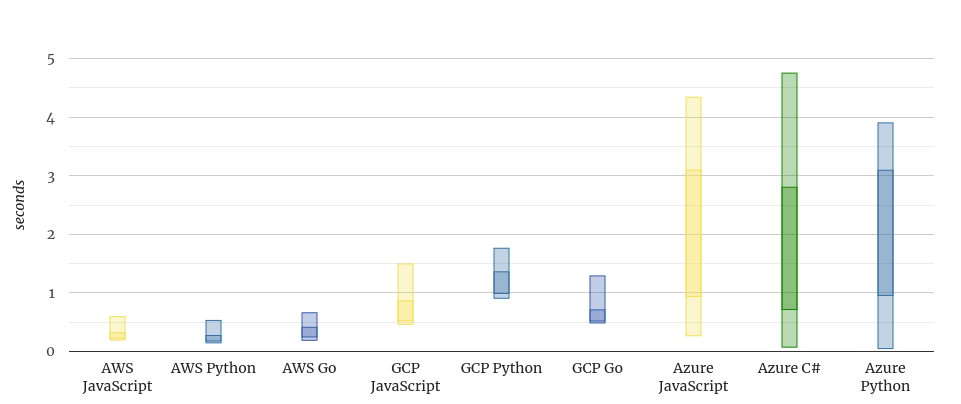
\includegraphics[width=\linewidth]{figs/ColdStart-programming-languages}
	\caption {اهمیت زبان و پلتفرم بدون سرور در تاخیر شروع سرد}
	\label{fig:ColdStart-programming-languages}
\end{figure}

\par
همانگونه که در تصویر \ref{fig:ColdStart-programming-languages} می‌بینیم، این آماده سازی شامل آماده سازی کانتینر‌ها، آماده سازی تابع، اختصاص منابع به کانتینر و در نهایت، اجرا در پلتفرم است. این تاخیر بسیار قابل توجه است و در شکل \ref{fig:coldstart-importance} نیز به خوبی نشان داده شده است. 

\par
همچنین،‌ یکی از مواردی که شروع سرد اتفاق می‌افتد، فراخوانی تابع برای اولین بار در پلتفرم است. 

حال چه عواملی در شروع سرد نقش دارند؟ عوامل عمده‌ای در این کار دخیل هستند ولی مهم‌ترین آن‌ها زبان برنامه‌نویسی و نوع پلتفرمی که در آن کد را اجرا می‌کنیم و کانفیگ نرم‌افزاری و سخت‌افزاری آن پلتفرم است. 

در مورد اهمیت زبان‌های برنامه نویسی می‌توان گفت چون زبان‌های مختلف زمان اجراهای متفاوتی دارند بنابراین موثر هستد. شکل زیر اهمیت زبان‌های برنامه‌نویسی را نشان می‌دهد. در این شکل از پلتفرم‌های مختلف برای اجرای توابع مختلف برای محاسبه‌ی زمان اجرا با درنظر گرفتن تاخیر شروع سرد استفاده شده است. 

در آزمایش دیگری با جاوا اسکریپت تابع‌های یکسانی نوشته شده با این تفاوت که حجم کتابخانه‌های هر تابع متفاوت است. این آزمایش در پلتفرم‌های مختلف نیز انجام شده و نتیجه طبق شکل زیر رسم شده است. 

\begin{figure}
	\centering
	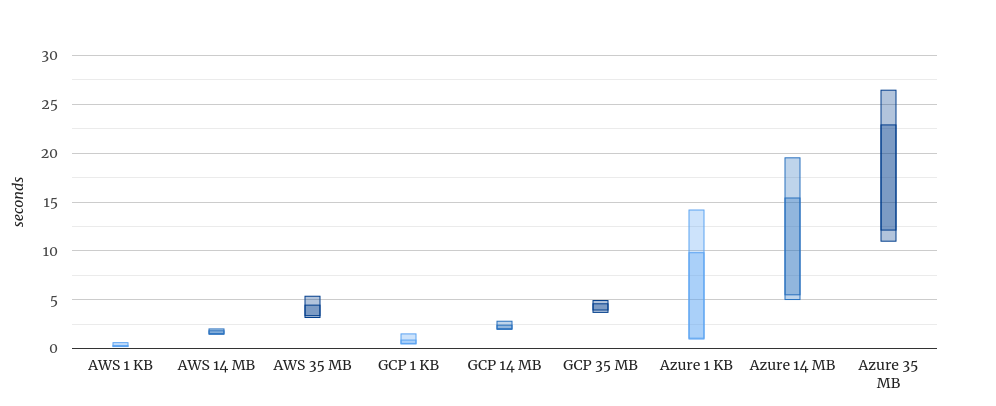
\includegraphics[width=\linewidth]{figs/ColdStart-programming-language-libraries}
	\caption {اهمیت اندازه کتابخانه برنامه  در تاخیر شروع سرد}
	\label{fig:ColdStart-programming-language-libraries}
\end{figure}

بنابراین با توجه به شکل \ref{fig:ColdStart-programming-language-libraries} می‌توان نتیجه گرفت حجم کتابخانه توابع نیز در مدت زمان تاخیر شروع سرد بسیار موثر است. 
\cchapter{کارهای مرتبط}
\label{related-works}

%%%%%%%%%%% معرفی Orchestration %%%%%%%%%%%%%%%%%%

قبل از بررسی درخت موضوعی بهتر است به مبجث ترکیب توابع در پلتفرم‌های بدون سرور بپردازیم. در \cite{bharti2021sequential} ۷ ترکیب  از توابع در FaaS بررسی شده است. البته این مقاله ذکر می‌کند که ۲ دسته‌بندی اصلی در رایانش بدون‌سرور داریم: \lr{MbaaS} و \lr{FaaS}. از \lr{MbaaS} به عنوان سرویس‌های سمت سرور برنامه‌های کاربردی وب و موبایل استفاده می‌کنند. پلتفرم Firebase یک نمونه از آن است. در حال حاضر این دسته‌از سرویس‌های ابری به شدت در حال توسعه است و البته، تمرکز این مقاله بر روی این موضوع هم نخواهد بود. 

یکی از چالش‌های اصلی معماری بدون سرور در ان است که برای تولید یک برنامه کاربردی بزرگ یا تجاری، باید جریان‌های کاری پیچیده‌ای را ایجاد کنیم. برای همین کار باید تعداد زیادی تابع را ایجاد کنیم که این توابع باید به اشکال مختلف هم‌دیگر را فراخوانی کنند. مثلا بعضا ممکن است یک تابع بعدی را فراخوانی کند یا یک تابع لازم باشد همزمان چند تابع را فراخوانی و اجرا کند و … . پیاده‌سازی یک راه حل درست برای این مورد بسیار برای رسیدن به معماری میکروسرویس برای ما مهم و حیاتی است و هرگونه کوتاهی و خطا در راه‌حل، باعث کارایی پایین محصول نهایی خواهد شد و با مشکلات بسیاری در پیاده‌سازی، ما را مواجه می‌سازد. 

برای حل این معضل، ارائه دهندگان خدمات تجاری اقدام به معرفی سرویس‌هایی تحت عنوان \lr{FaaS Orchestrator} نموده‌اند. هدف این سرویس‌ها ایجاد و پشتیبانی از ترکیب‌توابع و سناریو‌های پر‌کاربرد برای دستیابی به عملکرد روان در برنامه‌های کاربردی تحت پلتفرم بدون سرور است. دو پلتفرم معروف Orchestrator عبارتند از: \lr{AWS Step Functions} (با به اختصار \lr{ASF}) و دیگری \lr{IBM Cloud Function Sequences}.

توابع ترکیب شده توسط \lr{Orchestrator}ها حتما باید ۳ معیار را ارضا کنند: 

\begin{enumerate}
	
	\item ترکیبات توابع باید به‌ گونه‌ای باشند که جعبه سیاه بودن توابع نقض نشوند. یعنی فقط باید بتوانیم از روی ورودی و خروجی توابع محتوای آن را حدس زد.
	
	\item این ترکیب‌ها تابع قوانین و قواعد مشخصی باشند. همچنین، این ترکیبات باید قابل جایگزینی باشند.
	
	\item نباید بگونه‌ای فراخوانی اتفاق بیافتد که برای محاسبه‌ی هزینه همزمان پول ۲ تابع یا بیشتر را بدهیم\LTRfootnote{double billing}.
	
\end{enumerate} 

ما از این سه قانون با عنوان لم‌های بدون سرور\LTRfootnote{Serverless Trilemma} یاد می‌کنیم و هر ترکیبی از توابع که این ۳ معیار بالا را ارضا کند، \lr{ST-Safe} نامیده می‌شود. ترکیبات معروف توابع به شرح زیر است: 

\begin{enumerate}
	
	\item ترکیب با استفاده از بازتاب‌\LTRfootnote{Reflection}: به این صورت است که یک تابع اقدام فراخوانی سایر توابع به صورت همزمان \LTRfootnote{synchronous} می‌کند. در شکل \ref{fig:FaaS-Reflective-Pattern.png} یک نمونه مثال از فراخوانی همزمان توابع ذکر شده است. تنها مشکلی که دارد این است که با معضل \lr{Double billing} مواجه خواهیم شد. 
	
	\begin{figure}
		\centering
		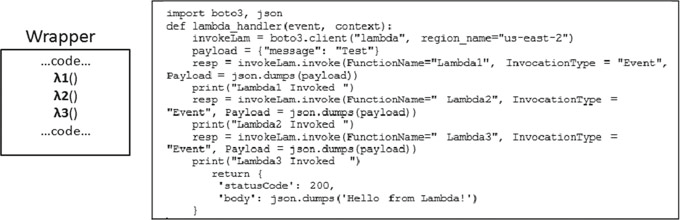
\includegraphics[width=\linewidth]{figs/FaaS-Reflective-Pattern.png}
		\caption {الگوی بازتابی در فراخوانی‌ها}
		\label{fig:FaaS-Reflective-Pattern.png}
	\end{figure}
	
	\item ترکیب همجوشی\LTRfootnote{Fusion} : در این حالت تابع \lr{wrapper}، توابعی که فراخوانی کرده‌ایم در تابع اصلی را بارگذاری می‌کند. مشکل اصلی آن این است که اصل جعبه سیاه را نقض می‌کند و همچنین باید توابع حتما با یک زبان نوشته شوند.  شکل \ref{fig:FaaS-Fusion-Pattern} یک الگوی همجوشی را نشان می‌دهد. 
	
	\begin{figure}
		\centering
		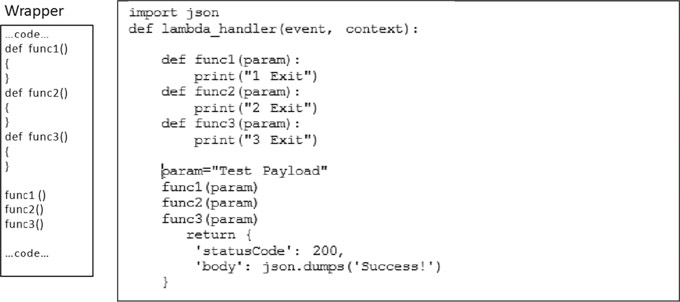
\includegraphics[width=\linewidth]{figs/FaaS-Fusion-Pattern}
		\caption {الگوی همجوشی در فراخوانی‌ها}
		\label{fig:FaaS-Fusion-Pattern}
	\end{figure}
	
	
	\item ترکیب غیرهمزمان: در این حالت،‌ تابع اول به فراخوانی تابع دوم می‌پردازد درحالی که اولی دیگر فعال نیست. این ترکیب نیز قانون دوم \lr{ST} را نقض می‌کند. 
	
	\item ترکیب توسط مشتری: در این حالت توابع ساخته می‌شود و خود مشتری خارج از سیستم بدون سرور اقدام به ترکیب توابع می‌کند. معروف ترین نمونه آن \lr{ASF} است و اصل اول را نقض می‌کند. 
	
	\item ترکیب زنجیره‌وار: در این ترکیب، یک ترکیب پس از اتمام اقدام به فراخوانی تابع بعدی می‌کند و همینطور ادامه پیدا می‌کند. این ترکیب مشکل \lr{double billing} دارد و \lr{ST-Safe} نیست. در شکل \ref{fig:FaaS-Chaining-Pattern} الگوی زنجیره‌ای نمایش داده‌شده است. 
	
	\begin{figure}
		\centering
		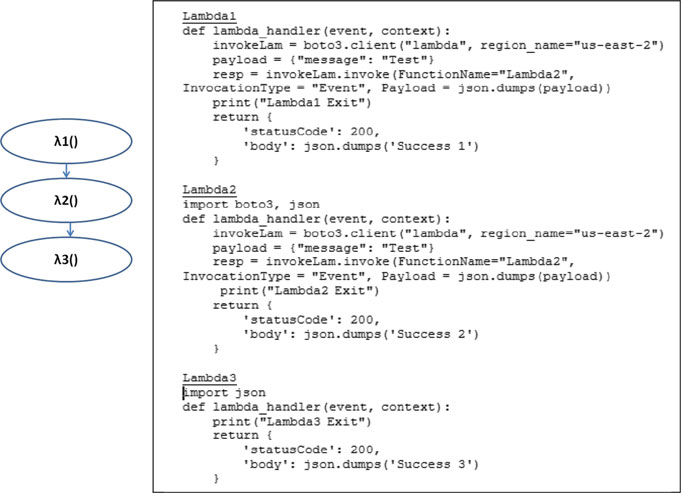
\includegraphics[width=\linewidth]{figs/FaaS-Chaining-Pattern}
		\caption {الگوی همجوشی در فراخوانی‌ها}
		\label{fig:FaaS-Chaining-Pattern}
	\end{figure}
	
\end{enumerate}

مقایسه‌ی این ترکیبات در جدول \ref{table:Function-Composition-Comparision} به طور خلاصه بیان شده است:‌

\begin{table}
	\caption{مقایسه‌ی بین روش‌های ترکیب توابع}
	\begin{center}
		
		\begin{tabular}{| c | c | c | c |}
			\hline
			نوع ترکیب & پشتیبانی از \lr{poly glot} & کدام محدودیت ST نقض می‌شود؟ & مدت زمان اجرای برنامه تست \\
			\hline
			بازتاب & بله & پرداخت مجدد\LTRfootnote{Double Billing} & $311.0.$ \\
			\hline 
			همجوشی & خیر & جعبه‌سیاه\LTRfootnote{‌Black Box} & $2.47$ \\
			\hline
			غیرهمزمانی\LTRfootnote{Async} & نامشخص & نامشخص & نامشخص \\
			\hline
			ترکیب توسط مشتری\LTRfootnote{Client}  & بله & قاعده ترکیب توابع & $331.83$ \\
			\hline
			زنجیره‌ای & بله & پرداخت مجدد & $1104.78$ \\
			\hline
		\end{tabular}
		\label{table:Function-Composition-Comparision}
	\end{center}
\end{table}

در نهایت با مقایسه دو پلتفرم \lr{ASF} و \lr{IBM Cloud Function Sequences} برای یک برنامه تست مشابه به مدت‌زمان ‌های اجرای شکل \ref{FaaS-Orchestrators-Comparision-Runtim} می‌رسیم. 

\begin{figure}
	\centering
	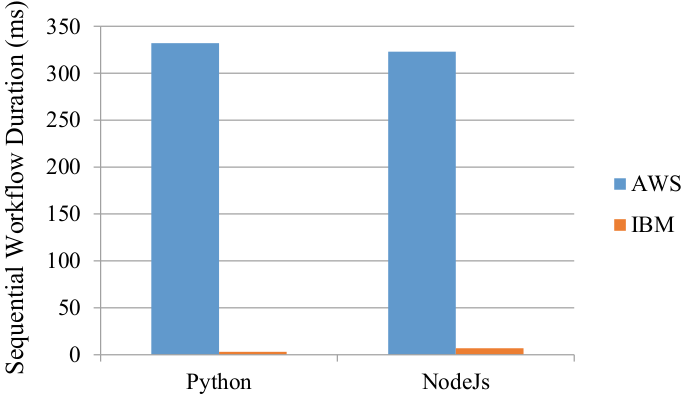
\includegraphics[width=\linewidth]{figs/FaaS-Orchestrators-Comparision-Runtime}
	\caption {مقایسه زمان اجرا ۲ برنامه مشابه با \lr{Node.js} و پایتون در دو پلتفرم \lr{ASF} و \lr{IBM Cloud Function Sequences}}
	\label{fig:FaaS-Orchestrators-Comparision-Runtime}
\end{figure}

%%%%%%%% درخت موضوعی %%%%%%%%%%%%%%%%%%%%%
\section{درخت موضوعی}

در این قسمت به بیان کارهای انجام شده در این حوزه خواهیم پرداخت و برای این کار درخت موضوعی مرتبط با آن رسم شده. هر گره ار درخت موضوعی یک راهکار برای جلوگیری از رخداد شروع سرد است و هر گره دارای بخش‌هایی است تا به برگ برسیم. در شکل \ref{fig:subject-tree} درخت موضوعی نمایش داده شده است و هر گره را به ترتیب بررسی خواهیم کرد. 

\begin{figure}
	\centering
	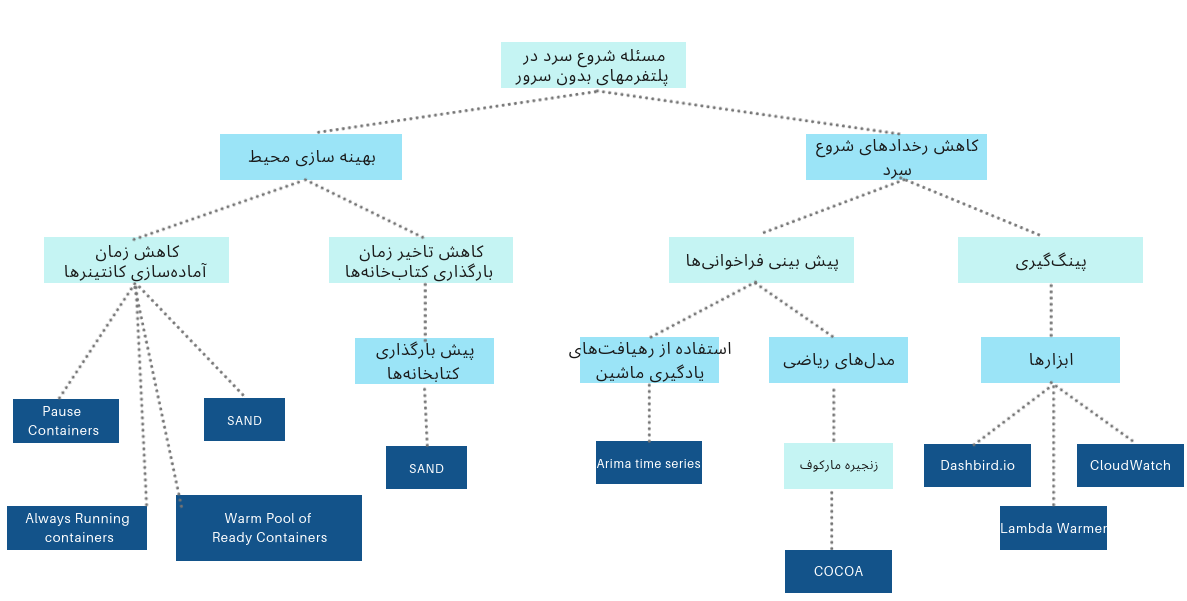
\includegraphics[width=\linewidth]{figs/subject-tree}
	\caption {درخت موضوعی}
	\label{fig:subject-tree}
\end{figure}

ریشه درخت مسئله شروع سرد است که ۲ گره اصلی دارد. گره سمت چپ که بهینه سازی محیط نام دارد، تلاش می‌کند تا در صورت وجود رخداد شروع سرد زمان آن‌را به حداقل برساند. این گره ۲ فرزند دارد که عبارتند از کاهش تاخیر آماده سازی کانتینرها و کاهش زمان بارگذاری کتابخانه‌ها. یک روش برای کاهش زمان بارگذاری کتاب‌خانه ها استفاده از روش پیش-بارگذاری است. 


گره سمت راست ریشه هم کاهش رخداد‌های شروع سرد است. تمرکز این گره در این است نگذاریم شروع سرد رخ دهد. گره سمت راست این نود، روش پینگ‌گیری است؛ در این روش سعی می‌کنیم با استفاده از ابزارهایی جلوگیری کنیم از سرد شدن توابع. در آخرین سطح این گره هم ابزارهای مرتبط معرفی شده‌اند. فرزند سمت چپ گره کاهش رخداد، پیش‌بینی فراخوانی‌ها است. در پیش‌بینی فراخوانی ها می‌توان از رهیافت‌های بدست آمده در یادگیری ماشین بهره جست. روش دیگر استفاده از مدل‌های ریاضیاتی غیریادگیری ماشین برای پیش‌بینی فراخوانی‌ها است. یکی از این روش‌های استفاده از ماشین‌ّهای حالت محدود بدست آمده با روش‌زنجیره مارکوف است.

 
در برگ‌های این درخت هرکدام یک مقاله را بررسی می‌کنیم. در ابتدا به توضیح درباره روش‌های بهینه‌سازی محیط می‌پردازیم و سپس به سراغ کاهش رخداد میرویم. در هر حوزه یک مقاله نمونه بررسی خواهد شد. 

\section{ بهینه سازی محیط}
          
          در این روش قرار به این است که مانع وقوع شروع سرد نشویم (در واقع هم نمی‌توان مانع از اتفاق شروع سرد شد)؛ بنابران به دنبال روش‌ یا روش‌هایی برای کاهش زمان شروع سرد هستیم. همانگونه که بالاتر ذکر کردیم، این موضوع را می‌توان از دو جنبه بررسی کرد. اول اینکه آماده‌سازی کانتینر‌ها را کاهش دهیم. روش دیگر این است که زمان لودشدن کتابخانه‌ها برای اجرای تابع را کاهش دهیم. برای این کار می‌شود از روش پیش-بارگذاری کتابخانه ها استفاده کرد.  
          
\subsection{کاهش زمان آماده‌سازی کانتینرها}

در این روش دنبال کمینه‌سازی زمان شروع سرد با استفاده از روش‌هایی برای کانفیگ بهینه محیط برای مواجهه با شروع سرد هستیم. عمده کارهایی که در این بخش انجام می‌دهیم در سطح شبکه یا کانتینر‌ها برای بهینه سازی است که روش‌های نسبتا سطح پایینی محسوب می‌شوند. 

یکی از مواردی که شروع سرد به شدت رخ می‌دهد، زمانی است که بنابه‌دلایلی تابع درخواست‌های زیادی دارد. این موضوع در \cite{lin2019mitigating} ذکر شده است. نویسنده معتقد با انجام این بهبودها در حدود 85٪ مدت‌زمان شروع سرد برای این توابع صرفه‌جویی خواهد شد. این مقاله از پلتفرم \lr{Knative} برای پیاده‌سازی تغییرات استفاده می‌کند. علت انتخاب \lr{Knative} این است که بر روی بستر کوبرنتیز ساخته می‌شود و از مفاهیمی مثل \lr{Pod} ها برای اجرای توابع و جریان‌های کاری استفاده می‌کند. بنابراین، از آنجایی که کوبرنتیز دست ما را برای انجام تغییرات باز می‌گذارد، می‌توان به آسانی به پیاده سازی سیاست‌های\LTRfootnote{policy} خودمان بپردازیم. در پلتفرم \lr{Knative} هر تابع در درون یک پاد اجرا می‌شود. پادها، ابتدایی‌ترین و ساده‌ترین بارهای‌کاری (به هر برنامه درحال اجرا در کوبرنتیز بارهای کاری می‌گوییم. توجه داشته باشید در کوبرنتیز بارکاری یک موجودیت نیست در واقع مفهومی است که به اجرای کانتینر‌ها و تخصیص \lr{CPU} و … اشاره دارد.) در کوبرنتیز هستند. در درون هر پاد تعدادی کانتینر اجرا می‌شود. در یک پاد شبکه‌ها، ذخیره سازی (Storage)‌ به صورت مشترک است. البته باز هم به خاطر وجود بحث‌هایی مثل \lr{Cgroups} و \lr{namespace} که ساختمان داده اصلی کانتینرها هستند، کانتینرهای داخل یک پاد از هم ایزوله هستند. پادهادر کوبرنتیز موجودیت‌های موقتی هستند و درصورت از دست رفتن نود، اتمام کار، کمبود منابع سرور و دلایل دیگر می‌توانند از سرور خارج شوند و دیگر قابل بازیابی نیستند. 

نکته‌ای که باید توجه داشت این است که یک پاد از جنس یک پردازه\LTRfootnote{Process} نیست؛ بلکه، محیطی منطقی برای اجرای کانتینر‌هاست و این کانتینرها هستند که از جنس پردازه‌ها هستند. داده‌های درون کانتینر‌ها وابسته به پادها هستند و با ری‌استارت شدن پادها محتویات ذخیره شده در کانتینرها از بین می‌روند مگر اینکه در ذخیره‌سازها ذخیره بشوند.\cite{KubernetesInAction}

با توجه به مقدماتی که در مورد پاد‌ها ذکر شد، اکنون منطقی به نظر می‌رسد برای مدیریت کانتینر‌ها بخواهیم از پادها استفاده کنیم و این رهیافت دست ما را برای اعمال تغییرات مختلف روی پلتفرم باز می‌کند. 

ما به صورت ایده‌آل دنبال کمترین سربار برای فراخوانی توابع هستیم. هنگامی که برای اولین بار تابع را فراخوانی می‌کنیم دچار تاخیر شروع سرد می‌شویم که در بخش ادبیات موضوع (رفرنس به شروع سرد)‌ در مورد آن مفصلا بحث کردیم. این مشکل در تمامی پلتفرم‌های بدون سرور، مشکل رایجی است. سربار شروع سرد را می‌توان به ۲ قسمت تعیین کرد :‌

\begin{enumerate}
	\item سربار ناشی از اجرای پلتفرم
	
علت اصلی این سربار اجرای پلتفرم است و به علت قرار گرفتن در صف یا دلایل دیگر باعث تاخیر می‌شود. از این دسته خطا‌ها می‌توان به network bootstraping، pod provisioning یا nework sidecar اشاره کرد. 
	
	\item سربار ناشی از خود اپلیکیشن
	
علت اصلی این سربار مشکلات خود برنامه است. این نوع تاخیر به مواردی از جمله زبان برنامه‌نویسی، حجم برنامه و نوع کتاب‌خانه‌هایی که از آن‌ها استفاده می‌کنیم بستگی دارد.
	
	
\end{enumerate}
 

برای مثال اجرای یک \lr{HTTP Server} ساده شروع سردی در حدود 5 ثانیه را به خود اختصاص می‌دهد؛ درحالی‌که با اجرای یک برنامه کلاس‌بندی عکس زمان شروع سرد به چیزی در حدود 40 ثانیه هم برسد. 

بنابراین، ایده این مقاله این است که برای اجرای توابعی که اخیرا محبوب شد‌ه‌اند از رهیافت استفاده از یک استخر گرم برای نگه‌داری این پاد استفاده‌کنیم. دقت کنید که در اینجا، در داخل هر پاد تنها یک کانتینر که آن کانتینر هم برای یک تابع است، اجرا می‌شود. هرگاه که درخواست جدید برای تابع می‌رسد در ابتدا استخر گرم را چک می‌کنیم که آیا پاد در آن موجود است یا خیر؟ اگر پاد در آن وجود داشت دیگر منتظر نمی‌مانیم، سریع تابع را در پلتفرم اجرا کرده و دیگر تاخیر شروع سرد را نخواهیم داشت. بنا به محاسبه نویسنده مقاله، این روش تا 85٪ زمان شروع سرد را برای توابع \lr{on-demand} نسبت به حالت عادی، کاهش می‌دهد. 

اما چگونه این تغییرات انجام شده است؟ شکل \ref{fig:knative-architecturea} نمایشگر معماری پلتفرم بدون سرور \lr{Knative} است. انتظار داریم با بهینه‌سازی‌هایی این رهیافت را برای مدیریت شروع‌های سرد اعمال کنیم. 

\begin{figure}
	\centering
	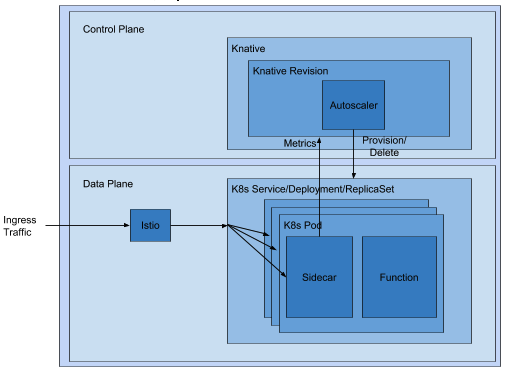
\includegraphics[width=\linewidth]{figs/knative-architecture}
	\caption {معماری پلتفرم Knative}
	\label{fig:knative-architecture}
\end{figure}

همانگونه که در این شکل می‌بینیم، وظیفه مولفه \lr{autoscaler}،  انجام وظایف مربوط به \lr{Scale up/down} است. هنگامی که دچار شروع سرد می‌شویم، مولفه \lr{autoscaler} دستور به ساخت پاد را می‌دهد  ولی از آنجایی که این امر وقت گیر است انجام آن بسیار طول می‌کشد. نهایتا اینکه پس از مدت زیادی پاد ساخته شده و داخل بخش \lr{data plane} اجرا می‌شود.

برای حل این مشکل، مقاله پیشنهاد می‌دهد تا در بخش \lr{control plane} و داخل \lr{revision} پلتفرم \lr{knative} یک مولفه مدیریت استخر قرار دهیم که آن با توجه به درخواست‌هایی که برای \lr{auto-scaler} می‌رسد، اقدام به ساخت پاد‌هایی و نگه‌داری آن در استخر گرم که در بخش \lr{data plane} توسعه داده شده، می‌کند. استخر گرم محدودیت ‌هایی مثل اندازه استخر دارد و تنها تعداد محدودی پاد در آن می‌توان نگه داشت.  حال اگر درخواستی برای پلتفرم برسد، \lr{autoscaler} ابتدا از کنترل کننده استخر\LTRfootnote{pool controller} وضعیت موجودی در استخر گرم را بررسی می‌کند. اگر در استخر پاد موجود باشد در اینصورت بلافاصله مهاجرت(migration)  از استخر گرم به سرویس رخ می‌دهد. از آنجایی که در استخر گرم منابع به پاد اختصاص داده شده و پاد کاملا آماده‌ی اجرا است؛ بنابراین، تاخیر شروع سرد بسیار ناچیزی خواهیم داشت. اما از طرفی، اگر پاد در استخر گرم موجود نباشد، دچار تاخیر شروع سرد خواهیم شد. نکته‌ی منفی این روش این است که در صورت رخداد شروع سرد، به میزان تاخیر‌های قبل، تاخیر ناشی از استعلام از استخر گرم ‌هم اضافه خواهد شد. شکل \ref{fig:Knative-architecture-modified} مدل جدید مقاله برای مدیریت شروع سرد را نشان می‌دهد. \cite{KubernetesInAction} 

\begin{figure}
	\centering
	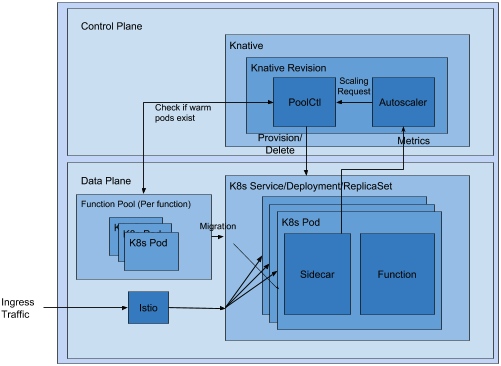
\includegraphics[width=\linewidth]{figs/Knative-architecture-modified}
	\caption {معماری پیشنهادی مقاله برای حل تاخیر شروع سرد}
	\label{fig:Knative-architecture-modified}
\end{figure}

\par
\par
مقاله دیگری که در این حوزه اقدام به بررسی تاثیر آماده سازی کانتیرها پرداخته از ایده pause container ها که مفهومی در کوبرنتیز است استفاده می‌کند. \ref{mohan2019agile}
این مقاله اقدام به بررسی تاخیر شروع سرد ناشی از اجرای همزمان تعدادی تابع کرد و نتایج خروجی آن را در شکل \ref{fig:coldstart-importance} نشان داده‌اند. 

در این واقع، این مقاله تاخیر شروع سرد را ناشی از آماده سازی کانتینر‌ها می‌بیند و سعی می‌کند تا حد امکان با آن مقابله کند. برای نمایش و پیاده‌سازی سناریو خود از پلتفرم‌ \lr{Apache OpenWhisk} استفاده کرده‌اند. طبق همان شکل نتیجه می‌گیریم که بخش عمده‌ای از تاخیرها ناشی از تاخیر در آماده‌سازی کانتینرها است، زیرا باید گام‌های طولانی برای ساخت و استقرار یک کانتینر و اختصاص شبکه به آن برداریم. شکل \ref{fig:container-network-creation} این گام ها را نشان می‌دهد.

\begin{figure}
	\centering
	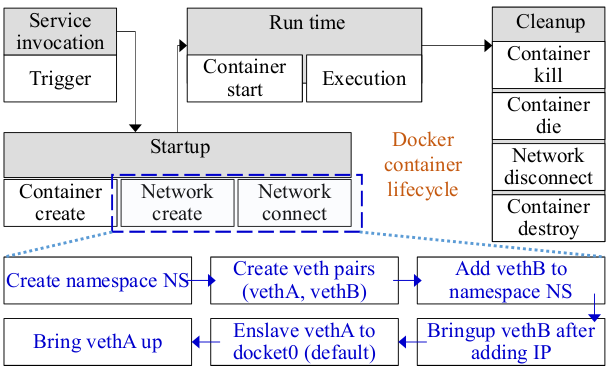
\includegraphics[width=\linewidth]{figs/container-network-creation}
	\caption {مراحل ساخت یک فضای نام در داکر}
	\label{fig:container-network-creation}
\end{figure}

همانگونه که در شکل مشخص است برای اجرای یک تابع در پلتفرم، ابتدا باید کانتیر آن ساخته شود. بسیاری از پلتفرم‌ها از جمله پلتفرم \lr{OpenWhisk} - که این مقاله تغییرات را بر بستر این پلتفرم بدون سرور انجام می‌دهد، - ازموتور داکر به عنوان موتنو کانتینری در پلتفرم خود پشتیبانی می‌کنند. در این موتور مراحل شکل فوق باید انجام بشود تا یک کانتینر کاملا آماده شود.

با توجه به شکل، تمامی بهبودهایی که باید انجام دهیم در مرحله شروع اولیه کانتینر است، جایی که دقیقا 3 مرحله داریم. ساخت کانتینرها، ساخت شبکه‌ها و اتصال کانتینرها به آن‌ها و در نهایت اتصال شبکه‌ها. 

در مرحله‌ای اول باید فضای نام‌را برای هر شبکه ایجاد کنیم. این کار در داکر توسط یک ویژگی کرنل لینوکس به نام فضای نام \LTRfootnote{namespace} انجام می‌گیرد. فضای نام یه مانع یا ایزوله کننده شبکه است که فرایند مختلف را از یکدیگر جدا می‌کند. در هر فضای نام پس از ایزوله سازی می‌توان مطمئن بود که دسترسی به پردازه‌های دیگر به شدت محدود شده است. اما، ما به دنبال ایزوله کردن پروسه نیستیم، بلکه به دنبال این هستیم که اجرا پردازه در سیستم عامل ایزوله باشد ولی ارتباط با آن نیز ممکن باشد. بنابراین باید تنظیمات شبکه در آن را انجام دهیم. 

بنابراین به دنبال ایجاد جفت‌های \lr{veth} \LTRfootnote{namespace} هستیم. جفت‌های \lr{veth} یک سری کابل مجازی هستند ( به طور دقیق از جنس خط لوله‌ها در سیستم عامل هستند) که وظیفه انتقال یک طرفه از کانتینر به فضای بیرون از آن و بالعکس را دارا می‌باشند. پس اقدام به اضافه کردن \lr{veth}ها به شبکه می‌کنیم. این دوقسمتی که مطرح شد خود شامل 6 مرحله کلی می‌شود که توضیح آن در این گزارش جایی ندارد.

حال نقش شبکه‌ها در شروع سرد چیست؟‌ همانگونه که قبلا گفتیم، هر کانتینر از 4 مرحله می‌گذرد. مرحله اول، مرحله فراخوانی سرویس هاست که در آن یک درخواست ساخت کانتینر برای \lr{docker daemon} ارسال می‌شود. مرحله دوم مرحله آغاز‌کردن\LTRfootnote{Startup} نام دارد که در طی آن یک کانتینر باید برای اتصال به محیط پیرامون آماده شود بنابراین کانتینر ساخته شده، شبکه درون و بیرون کانتینر کانفیگ می‌شود و به هم متصل می‌شوند.. مرحله سوم مرحله اجرا\LTRfootnote{execution} است که در طی آن، تابع اجرا می‌شود و در انتها مرحله‌ی نهایی یا مرحله پاکسازی\LTRfootnote{Cleanup} را داریم که شامل توقف اجرای کانتینر، قطع اتصال شبکه و نابود سازی آن است. \cite{DockerInAction}

علاوه ساخت کانتینرها،‌ به این توجه کنید که ما به دنبال اجرای همزمان آن‌ها نیز هستیم. این مورد زمان و سربار اجرا را نیز به طرز قابل توجهی بالا می‌برد.	اگر به شکل \ref{fig:coldstart-importance} نگاه کنید مجددا می‌بینید که به ازای اجرا‌های همزمان، زمان آماده‌سازی بسیار طولانی‌تر شده است درحالی‌که، زمان اجرا تغییر چندانی نکرده است. 

مقاله می‌گوید که بر طبق آمارهای گرفته شده، در مرحله آماده‌سازی کانتینرها، 90٪ زمان آماده‌سازی مربوط به ۲ مرحله ساخت شبکه‌ها و اتصال شبکه‌ها می‌شود. بنابراین معتقد است که با بهبود در این وضعیت تاخیر شروع سرد تا حد قابل توجهی برای تمامی توابع، کاهش خواهد یافت. حال مشکل اینجا‌است که این مراحل به کندی انجام می‌شوند مثلا برای ساخت شبکه این کار یکی یکی و در یک صف به نوبت انجام می‌شود. با توجه به اینکه در پلتفرم‌های بزرگ و تجاری در هر لحظه تعداد زیادی کانتینر باید ساخته یا حذف شوند این تاخیر به شدت افزایش پیدا خواهد کرد. برای اینکار آزمایشی انجام شد که نتایج آن در جدول \ref{table:1} قابل مشاهده است. 
\par

\begin{table}[h]
	\begin{center}
		\caption{زمان ساخت و پاکسازی کانتیرهای همزمان}
		\begin{tabular} {| c | c | c | c | c |}
			\hline
			
			تعداد فضا‌های نام همزمان & $1$ & $10$ & $50$ & $100$ \\
			\hline
			زمان ساخت & $0.28$ & $1.27$ & $6.28$ & $14.41$ \\
			\hline
			زمان پاکسازی & $0.20$ & $0.71$ & $3.24$ & $7.77$ \\
			\hline
		\end{tabular}
	\label{table:1}
	\end{center}
\end{table}

همانگونه که در این جدول قابل مشاهده است، زمان آماده‌سازی سرویس‌ها به ازای تعداد تعداد کانتینرهای همزمان، به طور نمایی افزایش می‌یابد. در حالی‌که ما در پلتفرم‌های تجاری همزمان تعداد زیادی کانتینر را هم بسازیم یا از بین ببریم. 

بهتر است به این دید نگاه کنیم که \lr{pause container} ها از قبل شبکه را ساخته و کانفیگ‌های مربوطه را انجام داده‌اند. پس کانتینری که در درون آن اجرا می‌شود تنها به معرفی برای اختصاص آدرس IP دارند که کار زمان‌بری نیست. بنابراین، می‌توان پس از ساخت یک کانتینر، تنها به اجرای آن در \lr{pause container} ها بپردازیم و از این طریق در زمان ساخت بسیار صرفه جویی کنیم. همچنین برای پاکسازی تنها باید کانتینر تابع مربوطه را حذف کنیم و \lr{pause container} بازیابی می‌شود. این رهیافت در شکل \ref{fig:pause-container-solution} نشان داده شده است.

\begin{figure}
	\centering
	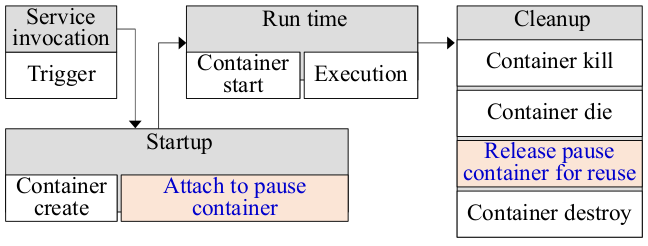
\includegraphics[width=0.8\linewidth]{figs/pause-container-solution}
	\caption {استفاده از \lr{Pause Container}ها برای کاهش تاخیر شروع سرد}
	\label{fig:pause-container-solution}
\end{figure}

در این حالت دو مرحله ساخت و اتصال شبکه جایگزین شده. همچنین برای مدیریت \lr{pause container} ها نیز یک استخر مربوط به آن‌ها ساخته‌شده است. در شکل \ref{fig:Pause-Container-Pool-Manager} نحوه عملکرد این رهیافت توضیح داده شده است.

\begin{figure}
	\centering
	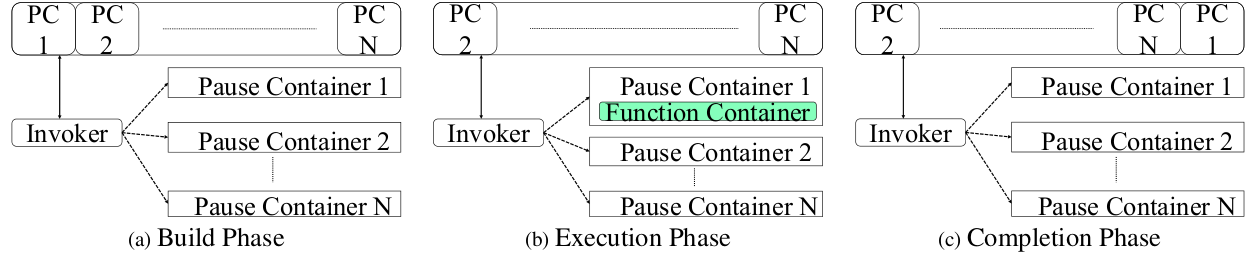
\includegraphics[width=\linewidth]{figs/Pause-Container-Pool-Manager}
	\caption {مدیر استخر \lr{Pause Container}ها}
	\label{fig:Pause-Container-Pool-Manager}
\end{figure}
 
در قسمت اول که فاز ساخت است۷ از قبل تعدادی کانتینر ساخته شده و در یک صف نگهداری می‌شوند. یک فراخواننده\LTRfootnote{invoker} داریم که وضعیت تمامی PC\LTRfootnote{مخفف Pause Container}ها را می‌داند. در قسمت بعدی می‌خواهیم یک تابع را اجرا کنیم؛ برای اینکار تنها کافی‌است که آن کانتینر را درون PC بارگذاری کنیم. و هرگاه کار تابع تمام شد تنها کافی است آن کانتینر در \lr{PC} را نابود کنیم. در انتها خود \lr{PC} بازیابی می‌شود و به انتهای صف استخرهای \lr{PC} اضافه می‌شود. 

نتایج این رهیافت در شکل زیر نشان داده شده است و می‌تواند تا 80٪ زمان شروع سرد را برای توابع کاهش دهد. برای مقایسه میزان بهبود داده شده شکل را با شکل مقایسه کنید.


\begin{figure}
	\centering
	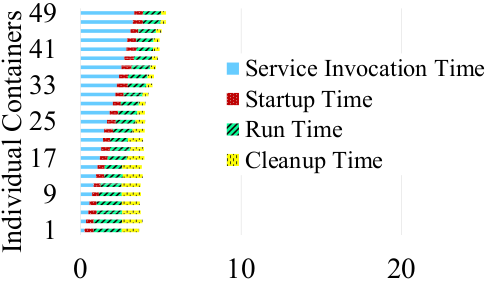
\includegraphics[width=0.8\linewidth]{figs/Pause-Containers-Results}
	\caption {نتیاج و بهبود حاصل شده با استفاده از \lr{Pause Container}ها}
	\label{fig:Pause-Containers-Results}
\end{figure}

%%%%%%%%%%%%%%%%%%%%%%% کاهش رخداد‌های شروع سرد%%%%%%%%%%%%%%%%%%%%%%%%%%%%%%%%%%%%

\section{کاهش رخداد‌های شروع سرد}

در این قسمت به دنبال روش‌هایی برای کاهش احتمال شروع سرد در پلتفرم‌های بدون سرور هستیم. در واقع ما به دنبال این هستیم که جلوی رخداد شروع سرد را با هایی بگیریم. از دسته‌بندی‌های کلی در این مبحث می‌وان به روش‌های جلوگیری از شروع سرد با استفاده از پینگ‌گیری یا روش‌های پیش‌بینی شروع سرد، اشاره کرد. 

\subsection{پینگ‌گیری}
متن تست
\subsubsection{استفاده از ابزار‌ها}
متن تست
\subsection{پیش‌بینی فراخوانی‌ها}
متن تست
\subsubsection{استفاده از مدل‌های ریاضی }
متن تست
\subsubsection{استفاده از رهیافت‌های یادگیری ماشین}
متن تست
\cchapter{نتیجه‌گیری}
\label{conclusion}

%%%%%%%%%%%%%%%%%%%%%%%%%%%%%ایده و محدوده کار آینده %%%%%%%%%%%%%%%%%%%%%%%%%%%%%%
\section{ایده و محدوده‌ی کاری در آینده}

با مطالعه در ادبیات موضوع\ref{literature} و کارهای انجام\ref{related-works}  شده فهمیدیم که مشکل شروع سرد مشکل گسترده‌ای است و محدود به حوزه‌ی خاصی نمی‌شود. همانگونه که مطرح شد عواملی مثل حجم حافظه مصرفی تابع، سربار تابع، نوع کانفیگ سرور، مشخصات سخت‌افزاری سرور زیرساخت، وضعیت شبکه، زبان برنامه‌نویسی‌ای که تابع با آن نوشته شده و ... در تاخیر شروع سرد بسیار موثر و تاثیرگذار هستند. البته در این گزارش از بی روش‌های کنترل شروع سرد بر روی ویژگی‌های شبکه برای کاهش مدت زمان آماده‌سازی و روش‌های پیشگیری از شروع سرد توقف کردیم. متاسفانه مدت زمان کافی برای مطالعه سایر روش‌ها فراهم نشد. 

روش‌های پیشگیری از شروع سرد، اگر چه در سناریوی موفق خود باعث به صفر رسیدن تاخیر شروع سرد می‌شوند، اما در سناریوهای ناموفق خود تاخیر شروع سرد به طور عادی برای تابع اتفاق می‌افتد. نکته‌ی منفی درمورد اکثر این روش‌های این است که علاوه‌بر دقت پایین یا خطا‌های بسیار برای شناسایی الگوی شروه سرد، - که کار بسیار دشواری هم هست، - این روش‌ها سربار محاسباتی بسیار بالایی برای پیش‌بینی دارند درحالی‌که وقت ما برای پیش بینی بسیار محدود است. از طرف دیگر، پیچیدگی اجرا و مدت‌زمان سربار محاسباتی برای روش‌های مبتنی بر کاهش زمان شروع سرد بسیار کمتر است. شاید به همین دلیل است که بیشتر در صنعت و پژوهش‌های عملی مورد استقبال قرار گرفته اند. از طرفی هم این روش ها مانع از تاخیر شروع سرد نمی‌شوند و نمی‌توانند به طور کامل جایگزین روش پیشگیری از شروع سرد شوند. 

به نظر می‌رسد ترکیب این دو روش به عنوان کار آینده گزینه جذابی باشد. مثلا از راهکار‌هایی برای فرار از شروع سرد استفاده کرد. در کنار این قضیه، از راهکارهایی نیز برای جلوگیری از شروع سرد استفاده کنیم. در بهترین حالت، علاوه بر اینکه زمان پاسخ را کم کرده‌ایم توانسته ایم با دقت خوبی هم از به وقوع پیوستن شروع سرد نیز جلوگیری کنیم. اما از طرفی ممکن است باعث بیش‌مهندسی\LTRfootnote{Over Engineering} شدن قضیه بشویم. این موضوع نیازمند بررسی بیشتر است و نیاز به تحقیق بیشتری برای قطعی شدن موضوع داریم. 

در قدم پیشرفته‌تر می‌توان از این کار برای به حداقل رسانی شروع سرد در ترکیبات توابع استفاده کرد. این موضوع برای به حداقل رسانی توابعی که در Orchestrator ترکیب شده‌اند بسیار مفید می‌تواند باشد. فرض کنید ۲ تابع داریم که با الگوی زنجیره‌ای\LTRfootnote{Chaining} به هم وصل شده‌اند. پس با فراخوانی تابع اول می‌دانیم تابع دوم هم حتما فراخوانی می‌شود. پس باید قبل از فراخوانی، تابع گرم شود. برای این کار پژوهش‌های انجام شده در \cite{mohan2019agile, lin2019mitigating} می‌تواند بسیار کمک کننده باشد. 

اگر قرار به استفاده از دیتاستی باشد تنها دیتاست در دسترس در \cite{AzurePublicDataset} وجود دارد که اطلاعات مصرف و فراخوانی توابع در سال‌های 2019 و 2020 را به صورت متن‌باز منتشر کرده‌است. برای این کار مجبور هستیم اقدام به پیاده‌سازی پلتفرم مد نظر خود کنیم. برای این کار احتمالا مجبور شویم کدپروژه پلتفرمی را که می‌خواهیم تغییر دهیم را برای سازگاری با سیاست‌های خودمان تغییر دهیم. نتیجه این تغییرات پلتفرم جدیدی بر مبنای پلتفرم پایه خواهد بود که آن را در آینده ارائه خواهیم داد. 










%%%%%%%%%%%%%%%%%%% نتیجه گیری کلی %%%%%%%%%%%%%%%%%%%%%%%%%%
\section{نتیجه‌گیری کلی}

در \autoref{intro} به بیان مقدمه‌ای از موضوع و در \autoref{literature} به بیان ادبیات موضوع پرداختیم تا خواننده را با موضوعاتی که قرار است در پژوهش در باره آن بحث کنیم آشنا سازیم. پس از آشنایی با مباحث پایه‌ای به بیان کارهای انجام شده و ایده‌هایی که تاکنون در این حوزه مطرح شده است، در \autoref{related-works} پرداختیم. 

به طور خلاصه برای مدیریت شروع سرد دو سیاست کلی می‌توان داشت. سیاست اول این است که زمان آماده‌سازی برنامه را کم کنیم تا مدت زمان تاخیر به حداقل برسد. یعنی در واقع، ما اجازه وقوع شروع سرد را به تابع می‌دهیم ولی مدت‌ زمان ناشی از تغییر را حداقل کرده‌ایم. سیاست دوم این است که مانع وقوع شروع سرد بشویم. هر دو سیاست از موضوعات ترند و پرپژوهش در این حوزه هستند. 

همانگونه که می‌دانید روش پایه‌ای برای مدیریت شروع سرد، روش زمان ثابت زنده ماندن توابع\LTRfootnote{Fixed-Time alive} است. در این روش، تابع تا مدت زمان ثابتی پس از آخرین فراخوانی گرم می‌ماند و اگر در آن بازه صدا زده نشود سرد می‌شد. این روش بسیر ابتدایی است و هرگز نمی‌توانست الگو‌های فراخوانی را تشخصی دهد و در فراخوانی‌های متناوب در بازه‌های طولانی‌تر از بازه \lr{Keep Alive}، همواره شروع سرد را تجربه می‌کردیم. اگرچه در مصرف منابع هم به نسبت بازدهی خوبی نداریم. بنابراین این روش در مقایسه با روش‌هایی که به دنبال مدل‌سازی برای گرم کردن تابع هستند نه بازدهی خوبی از نظر منابع دارد و نه توانسته است از نظر مدت‌زمان پاسخ\LTRfootnote{Response Time} پاسخ خوبی داشته باشد. 

از طرفی روش‌های بهینه‌سازی سرور وجود دارند که اگرچه مدت زمان پاسخ با درنظر گرفتن شروع سرد را کاهش می‌دهند اما خود باید مراقب سربارهای احتمالی مانند سایز حافظه کش، سایز استخر گرم و ... باشند تا بتوان گفت از نظر مصرف منابع بسیار بهینه عمل می‌کنند. این روش‌ّا اگر چه مدت زمان را کم می‌کند اما همچنان از تاخیر شروع سرد رنج می‌بریم. همچنین مدت‌زمانی که زمان پاسخ برمی‌گردد آن‌قدر کاهش نمی‌یابد که بگوییم مشکل زمان پاسخ حل شده است.

حال ایده‌ای که مطرح می‌شود این است که آیا با ترکیب این روش‌ها می‌توان به روش‌ بهینه‌ای برای مدیریت شروع‌های سرد رسید یا خیر؟‌ این سوال اصلی این پژوهش است و برای پاسخ به آن به مطالعه‌ی خیلی بیشتری نیاز است. اما اگر بتوانیم با استفاده از مدل پیشگیری مناسب مانع اتقاق افتادن شروع‌های سرد شویم و از ظرف دیگر با استفاده از یک تکنیک بهینه مدت زمان لود شدن تابع را حتی در صورت اتفاق افتادن شروع سرد کاهش بدهیم مسئله را با دقت بسیار خوبی حل کرده ایم.

البته باید توجه داشت این یک کار بسیار چالش برانگیز است. در \cite{gias2020cocoa} ماباید برای هر تابع بتوانیم زنجیره مارکوف آن را رسم کرده و با ترکیب با LQN به پیش‌بینی بهینه بر اساس توافقات سطح سرویس شویم. اینکار بسیار طولانی و چالشی است؛‌اگرچه که دقت خوبی دارد و به خوبی توانسته است سطح انتظارات را برآورده سازد. یا مثلا در \cite{shahrad2020serverless} ممکن است حتی مسئله را اصطلاحا بیش‌ مهندسی کرده باشیم. 

ما همواره در مهندسی نرم‌افزار و شبکه به دنبال کم کردن تاخیر ناشی از ارتباطات در شبکه و سرور با کاربران هسنیم. پس می‌توان گفت تا کنون به مبحث شروع سرد بسیار بی‌توجهی شده است. موضوع دیگری که در این بیین بسیار مغوف مانده است، امکان کاهش شروع سرد برای رکیبات توابع است که پاسخی برای این موضوع مشاهده نشده است. 







%%%%%%%%%%%%%%%%%%%%%%%%%%%
	
%%%%%%%%%%%%%%%%%%%%%%%%
% مراجع
\newpage
%\onehalfspacing
\bibliographystyle{ieeetr-fa}%{plainnat-fa}%{chicago-fa}%
\bibliography{thesis-copy}
%%%%%%%%%%%%%%%%%%%%%%%%

\end{document}
